\chapter{Description of the developed functionalities}
In order to expand the use of the BW4T environment, new functionalities were added. These functionalities will make it possible to create more diverse simulations for testing team strategies. In this chapter we describe how the new functionalities are implemented.

\section{Logger}

We extended an already existing functionality, namely the Logger. Originally the name of the log files were not very clear, for example 'BW4T748554815099389365.txt’. These names are not giving the users any information about what they’ve logged. Now the log files get the name of the date and time when the server is started. The format equals 'BW4T-year-month-day-hour.minute.second.log’, an example of a name of a log file: 'BW4T-2014-06-20-10.47.54.log’.

When pushing the reset button a new sequence will appear and the client needs to be restarted. The already existing log file will get a .1 after .log, when the reset button is pushed again, this .1 will turn into a .2. So when having multiple log files with same timestamp, the oldest log files will have the highest numbers. Within the log file we added a timestamp as well. Every time something is logged, the time of logging will be added.

At the end of the file a summary will be logged. Originally, the time that the sequence was finish was logged, but if you wanted to know how much time it took to complete the sequence you had to calculate it yourself. To make this easier, the logger now does this for you. When it took more than a minute to finish the sequence, the total minutes and seconds will be logged. If it took less than a minute the seconds and milliseconds will be logged. Furthermore, the original log files always mentioned that the type of a bot was unknown. Now, the handicaps will be printed or 'none' if the bot has no handicaps. Another issue was that the original logger did not log the amount of room entries per bot correctly. When a bot entered a room, the logger registered that the bot entered that room more than 10 times. When the bot left the room the logger also registered that the bot entered that room. We fixed this and now the number of rooms entered is correct.

\section{Scenario Editor}

The Scenario Editor (Figure ~\ref{fig:scenarioEditor}) is a new feature with which a configuration file can be created, opened, modified, saved and exported as a mas2g working directory. The editor can be divided into two main parts: The configuration panel and the entity panel.
In the toolbar there is a button "File". When clicked a drop down menu will appear with the options to open, create, save and export the file. Exiting the editor is also possible here.

To implement the Scenario Editor we made use of the MVC structure.

\begin{figure}
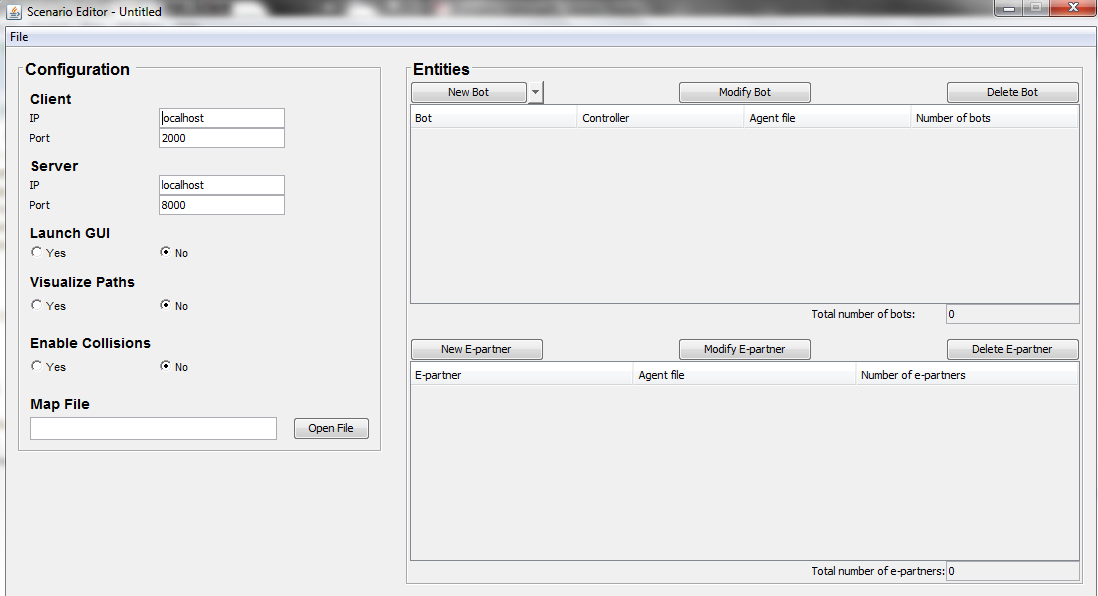
\includegraphics[width=\textwidth]{pictures/scenario-editor.png}
\caption{Scenario Editor}
\label{fig:scenarioEditor}
\end{figure}

\subsection*{Configuration panel}
Here, the client and server IP address and port number can be set. It can also be specified whether the GUI needs to be launched, whether the paths will be visualized and whether collisions will be enabled. Lastly, selecting a map file to use in the configuration is possible.

\subsection*{Entity Panel}
The bots can be created, modified and deleted here with the following three buttons: "New Bot", "Modify Bot" and "Delete Bot". Next to the "New Bot" button there is a drop-down button. Here you can add a new default bot to the bot list, which is being displayed below these three buttons. On the right side, under the bot list, the total number of bots is shown.

Below this, there are the three e-partner buttons, followed by the e-partner list and the total amount of e-partners created. It has the same functionalities as the bots part, but then for the e-partner.

By selecting a bot or e-partner and then clicking on the modify bot or e-partner button, the Bot Store or E-Partner Store will open. Here you can further configure your bot or e-partner.

\section{Bot Store}
In the Bot Store a bot can me modified to the users wishes. A standard bot is the most capable bot, meaning it does not have any handicaps. The handicaps are discussed after this. Several handicaps can be added to a bot. This way the user can adjust what a bot can or cannot do. Besides the handicaps the user can specify how fast a bot can go and what capacity the batter of the bot has. Also bots can now have different sizes. The speed, battery capacity and size can be adjusted with the sliders. When satisfied the save button is clicked and the custom bot settings are saved. 

\section{Handicaps}
Part of the functionalities that we have developed is that robots in BW4T can now have certain abilities and inabilities, also referred to as handicaps, to broaden the possibilities of types of simulations.

The first handicap that we have developed is the gripper handicap, allowing us to set the number of grippers of a robot in a range from 0 to 5, allowing it to hold up to that number of blocks simultaneously.

The second handicap is the handicap of color blindness, making the robot unable to distinguish colors of different blocks. This handicap still allows to robot to see the blocks but it will make all blocks appear as dark gray blocks, simulating a robot with a black and white camera.
Besides adding handicaps to a robot we can now also set different properties of the robot. In the scenario editor we can change the size and speed of the robot, creating a robot that is unable to pass through doors because it is simply too large for the door, or making a really fast bot that can walk through the map at a much higher speed than other bots, possibly serving as a robot purely meant to scan the map and tell robots with multiple grippers where certain blocks are.

The last feature we have added to the robots is that robots can now carry a battery with them. The original bots can always continue walking around the map, picking up blocks and talking to their team members. However, when the user now chooses to set a battery for a robot (enabling it in the scenario editor) it can set its capacity and the bot will run out of it after moving around the map for a period of time. It can then recharge its battery by finding its way to a charging zone and recharge it by walking over or standing on the charging zone. When the battery capacity is disabled the robot will always be able to keep moving.

\section{E-partner}
A feature that one customer specifically requested us to do was to implement an E-partner. An E-partner is a device similar to a tablet to support the robot.The E-partner is available to a robot in the corridors. It can have two functions. First it can have a gps function. With this function the E-partner checks wether or not the bot is going in the direction that it should. If the bot goes into the wrong direction it gives a notification that the bot should change its course. The second function the E-partner has is that it can detect if a bot puts it down and leaves the room. When this happens another notification is sent to the bot to inform it that it has forgotten the E-partner and it should head back to pick it up again. These two function can be selected in the E-partner store. When the right selections are made the E-partner can be saved with the save button.

\section{Environment Store}
The old map editor has been completely redesigned to what we now call the Environment Store. In this new Environment Store we are no longer limited to the standard mapping of rows and columns, bordered and separated by corridors with the start and drop zone at the bottom of the map. It offers the user the ability to create much larger maps and place the different types of zones across the map according to a grouping that is preferred by the user. \\

Besides the new functionality that allows us to position the door of a room on any side, we can now also add two new types of zones called blockades and charging zones. The blockades serve to create a map with parts where the robot cannot pass through. This way the user can create a maze that is difficult to navigate or zones that take a long time to reach. We have added charging zones which allow the bots that contain a battery to recharge when passing it. A charging zone is like an open space and does not contain any walls or doors. Both blockades and charging zones are the size of a basic room or corridor and therefore easily fit in the new mapping.
In the new Environment Store we allow the user to randomize every aspect of the new map separately. Through the tools menu the user can randomize the rooms through a standard algorithm or randomize the blocks in rooms and sequence according to parameters the user can set himself. This way a complete map can be generated within seconds, even if the map is as large as a 1000 editable zones. \\

After the user has created a map, or while editing a map, it can at any time show a live preview of the real map by using the `Preview Map' option in the `File' menu. This way the user can see how the changes in the map affect the actual environment as it would run in BW4T. When the user is satisfied with the map he has created, or simply wants to save the created map as a draft to continue with at a later stage, he can save and later open the map through a few simple clicks in the `File' menu.

\section{Human Player GUI}
One of the functionalities we have extended is the Human Player GUI (Figure ~\ref{fig:hpg}). We roughly split the interface up in two sections. The map is being displayed on the left, while the chat sessions are being displayed on the right.

\begin{figure}
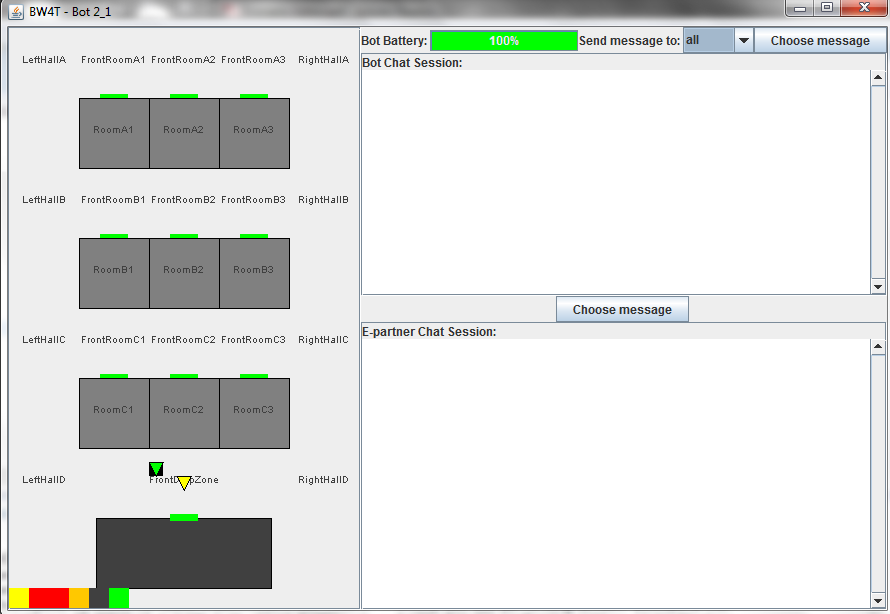
\includegraphics[width=\textwidth]{pictures/hpg.png}
\caption{Human Player GUI}
\label{fig:hpg}
\end{figure}

\subsection*{The map}
In the map there is the possibility to zoom in and zoom out with the mouse scroll button. There is also a scrollbar, which will appear when the map is larger than the area where the map is being displayed. Upon clicking on the rooms, corridors, blocks and/or e-partners, a drop-down menu will appear with the possible actions.

\subsection*{Chat sessions}
Originally there was only one chat session, but because of the addition of the e-partners, we have decided to split up the chat session into two chat sessions. One for bots to bots and one for bot to e-partner.

The bot battery is being displayed first. Next to it, there is a drop-down box where the user can select to which agent he/she wants to send a message to. There is also a button: `Send Message', where you can select the message to send. Below this, there is the chat session box of the bots. A drop-down menu with possible answers to questions will appear when clicked in the box. \\

Some space is reserved for the e-partner chat session and message button below the bot chat sessions. These will only appear when an e-partner is being held by the bot. As soon as the e-partner is dropped, the message button of the e-partner will disappear. The chat box will not disappear though. This way the e-partner can still send messages to the bot, if it has GPS enabled. The message button is only used for sending messages to the e-partner and dropping the e-partner.

\section{Collisions}
\subsection*{Features}
With the addition of collisions a few new features are available in BW4T. In this section a list of these features will be presented, along with a short description of said feature.

\begin{description}
	\item[Feature: Collisions] \hfill \\
		It is now possible for bots to collide with each other. This option can be toggled on and off.
	\item[Percept: bumped] \hfill \\
		When a collision occurs a bumped percept is sent to the bot who caused the collision. The bumped percept contains the name of the bot being bumped into.
	\item[Action: navigateObstacles] \hfill \\
		When a collision the navigateObstacles/0 action can be used to request a new path from the path planner, taking blocked tiles into account.
	\item[Feature: Visualize Paths]
		The paths being traversed by the bots can be made visible on the server display. 
	\item[Feature: Improved Path-finding]
		There are two pathfinders, one that uses the map zones as navigation points, and the new one which uses the grid points. 
\end{description}
		
\subsection*{Justification}
BW4T3 introduces the ability to collide with other bots on the map. Before version 3 there were no collision detection and handling methods, due to this bots were free to move through each other as they traversed the map. Before collisions could be enabled a few key issues had to be solved. In this section these issues will be discussed and the reasoning behind specific design decisions explained. \\

The main issue faced when planning the implementation of collision was that the path planner inherently could not handle collisions. In fact, the path planner as it is, is the main reason there are collisions. Currently all paths go through the center of each zone. Thus when traversing from A to C, all bots on that route will move through the center of B, thus creating a bottleneck. Furthermore, as the path planner only used the center of each zone, collisions could not be avoided if they were in the way to the center of a zone.
Therefore it was decided that a new path planner had to be implemented. This new path planner would not use the center of the map zones as navigation points, rather the points on the grid. To clarify, the map seen when the server is running displays the map zones. These can be rooms, corridors, drop zones, etc. All objects (e.g. zones) present on the map are located on an `invisible' grid. The new path planner uses the points on this grid as its vertices, with the points on the north, south, east and west as neighboring vertices, connected by an edge with length 1. 
While in theory vertical neighbors could be supported, they were not added as they are infinitesimally many, and would complicate collision detection.  \\

With the path planner created the next issue was detecting if a bot was going to collide with another bot or not. The original specifications called for a bumped percept to be called after a bot collided with another bot. Since implementing this would take as much effort as detecting a collision before it happened it was decided to detect collisions before they actually happen. In a way this is more realistic, as generally preventing a collision is the preferable solution. \\

When a collision is detected the `navigateObstacles' action can be used to plan a path around the obstacle. This action must be called separately. The action is not automatically called when an obstacle is detected, as it would remove the possibility for the agents to coordinate a plan to go around an obstacle. (Especially if two agents are blocking each others path). Note: When a collision occurs the agent can also use the goTo actions to go to a new location provided the path is free. \\

During the development of the collision features debugging proved quite complicated as there was no way to visually see the path generated. The solution was to draw the path on the map. This debugging tool proved quite handy during simulations, as it could be used to see how to bot reacted when a collision occurred. While it may not have any scientific value as it is purely visual, it has been included in BW4T3. It could be a helpful debugging aide, especially for 1st year students following the AI course, as it can be used to debug and visualize the actions of the robots. \\

A key improvement in BW4T3 was the complete and absolute separation of the client and server. In accordance with this it is possible to turn collision detection on/off  by setting the appropriate option in the Scenario Editor. However, it is also possible to change this setting on the server (and thus modifying the scenario loaded by the client). While this is in stride with the decision to fully separate the server and the client, it was decided to include the option on the server to make it easier to test environments with collisions enabled. This to avoid having to change the scenario and reload it on the server as this would be extremely cumbersome. By simply checking a box to have collisions be enabled or disabled this process was made significantly easier.

\subsection*{Current Concerns}
At the moment there is an issue that prevents the startup of bots on top of each other when collisions are enabled. Due to the complexity of writing a procedure that makes sure every bot spawns on an unoccupied location, it had been decided that for all bots collisions will be disabled for as long as, after they have spawned, they share a grid point with another bot. 
However, when using GOAL, somewhere during the initialization of Repast one of the navigating robots is presumably being cloned. But this happens after the robots are initially loaded into the context. Due to this, when the NavigatingRobot requests its location a null pointer is returned. This only happens when one robot is stepped before the other, with collisions enabled and two bots being on top of each other. Despite meticulously searching for the cause it could not be located. However, a simple workaround exists. To prevent this error from occurring one must, after initializing the environment, run the server for at least one step.

\section{Refactor}
We improved the quality of the code and the overall structure of the project by implementing the following:

\begin{itemize}
\item
\textbf{Split up codebase into Client and Server} - The client and server shared the same codebase. This made it hard to keep a proper overview as it wasn't always clear at a glance which class belonged to which subsystem, and some classes were even shared entirely. We split these subsystems into individual projects to make it easier to maintain, extend and test them. New features like the Map Editor and Scenario GUI were also added as separate projects. It turned out we couldn't cut all dependencies between the projects. For that reason, we created a shared library project as well, called the BW4T-core. 
\item
\textbf{Convert to maven project} - Maven is a build automation tool. It makes building and testing the project easier because it shields you from many of the details. It replaces the current complicated ANT buildscript, and accounts for dependencies. Maven provides guidelines for best practices, which is useful for large projects which can become very complex easily, like BW4T. Using Maven, it becomes much simpler to maintain a continuous working project.
\item
\textbf{Improve overall code quality} - Using source code analysis tools like Sonar and inFocus, we discovered that there were a lot of code quality issues present in the existing BW4T codebase.

\begin{itemize}
\item
There were a lot of very complex methods and classes. We reduced complexity to make the code easier to understand, maintain and extend. Cyclomatic complexity of methods now rarely exceeds 10 with an average of 1.8 per function, while class complexity doesn't exceed 159 with an average of 10.4. This reduction makes the code perform better, allows for easier extension and improves readability. 
\item
In order to make the code more readable, we applied a well-defined Checkstyle throughout the project. This included the use of curly braces and indentation, in order to prevent silly bugs from being created by missing braces and the likes.
\item
Javadoc was occasionally present, but often times contained insufficient information. We not only made sure that Javadoc was present for all relevant methods and classes, but also improved existing Javadoc so one is able to easily figure out what a method or class does without needing to read the actual code.
\end{itemize}

\item
\textbf{Add sufficient tests} - There were no tests present whatsoever in the old codebase. In order to ensure functionality after changes, a lot of tests have been written. We achieved 50\% line coverage for existing code, and 75\% line coverage for newly written code. 
\end{itemize}
